\section{Fragen zur Vorlesung -- Programmschnittstellen}

\begin{enumerate}[a)]
	\item Welche Vor- und Nachteile bringt die Verwendung eines Vorübersetzers zur Einbettung von SQL-Abfragen in Programmcode mit sich?

	\begin{solution}
	Vorteile:
	\begin{itemize}
		\item Kompakt zu programmieren.
		\item SQL-Anweisung wird zur Compile-Zeit geprüft, analysiert, optimiert, daher schnell und viele Fehler können schon zur Übersetzungszeit gefunden werden.
	\end{itemize}
	Nachteile:
	\begin{itemize}
		\item Spezieller Vorübersetzer für die Kombination aus Programmiersprache und DBMS notwendig.
		\item Häufig kein Standard-SQL, sondern mit syntaktischen Änderungen.
	\end{itemize}
	\end{solution}

	\begin{note}
	\begin{center}
	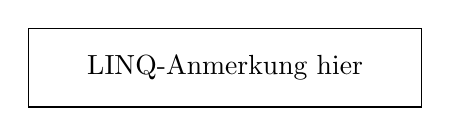
\begin{tikzpicture}
		\draw (0, 0) rectangle+(5, 1);
		\node at (2.5, 0.5) {LINQ-Anmerkung hier};
	\end{tikzpicture}
	\end{center}
	\end{note}

	\item Warum benötigt man bei Datenbankzugriffen aus Programmcode heraus in der Regel Cursor?

	\begin{solution}
	Da Programme im Allgemeinen mit einzelnen Werten arbeiten, Datenbanken aber mit einer Mengensemantik, ist es in der Regel so, dass Anfragen eine Ergebnismenge zurückliefern und nicht einzelne Werte.
	Um diese verarbeiten zu können, benötigt man eine Art Schleife über der Ergebnismenge, dies ist der Cursor. Mit diesem wird die Ergebnismenge in der Regel zeilenweise abgearbeitet; wobei nun jede Zeile in einzelne Werte zerlegt werden kann (Stichwort for-each-Schleife).
	\end{solution}

\end{enumerate}